\documentclass[a4paper, 11pt]{article}
\usepackage{comment} 
\usepackage{fullpage}
\usepackage{amsmath} 
\usepackage{amssymb} 
\usepackage{mathtools}
\usepackage{fontspec}
\defaultfontfeatures{Ligatures=TeX}
\usepackage{xfrac}
\usepackage{icomma}
\usepackage[section,below]{placeins}
\usepackage[labelfont=bf,font=small,width=0.9\textwidth]{caption}
\usepackage{subcaption}
\usepackage{graphicx}
\usepackage{grffile}
\usepackage{float}
\floatplacement{figure}{htbp}
\floatplacement{table}{htbp}
\usepackage{booktabs}
\usepackage{hyperref}
\usepackage[ngerman]{babel}
\begin{document}
\noindent
\centerline{\small{\textsc{Technische Universität Dortmund}}} \\
\large{\textbf{1. Übungsblatt zur Vorlesung \hfill WS 2017/2018 \\
Statistische Methoden der Datenanalyse \hfill Prof. W. Rhode}} \\
Annika Burkowitz, Sebastian Bange, Alexander Harnisch \\
\noindent\makebox[\linewidth]{\rule{\textwidth}{0.4pt}}

\section*{Aufgabe 1}
\begin{figure}
    \centering
    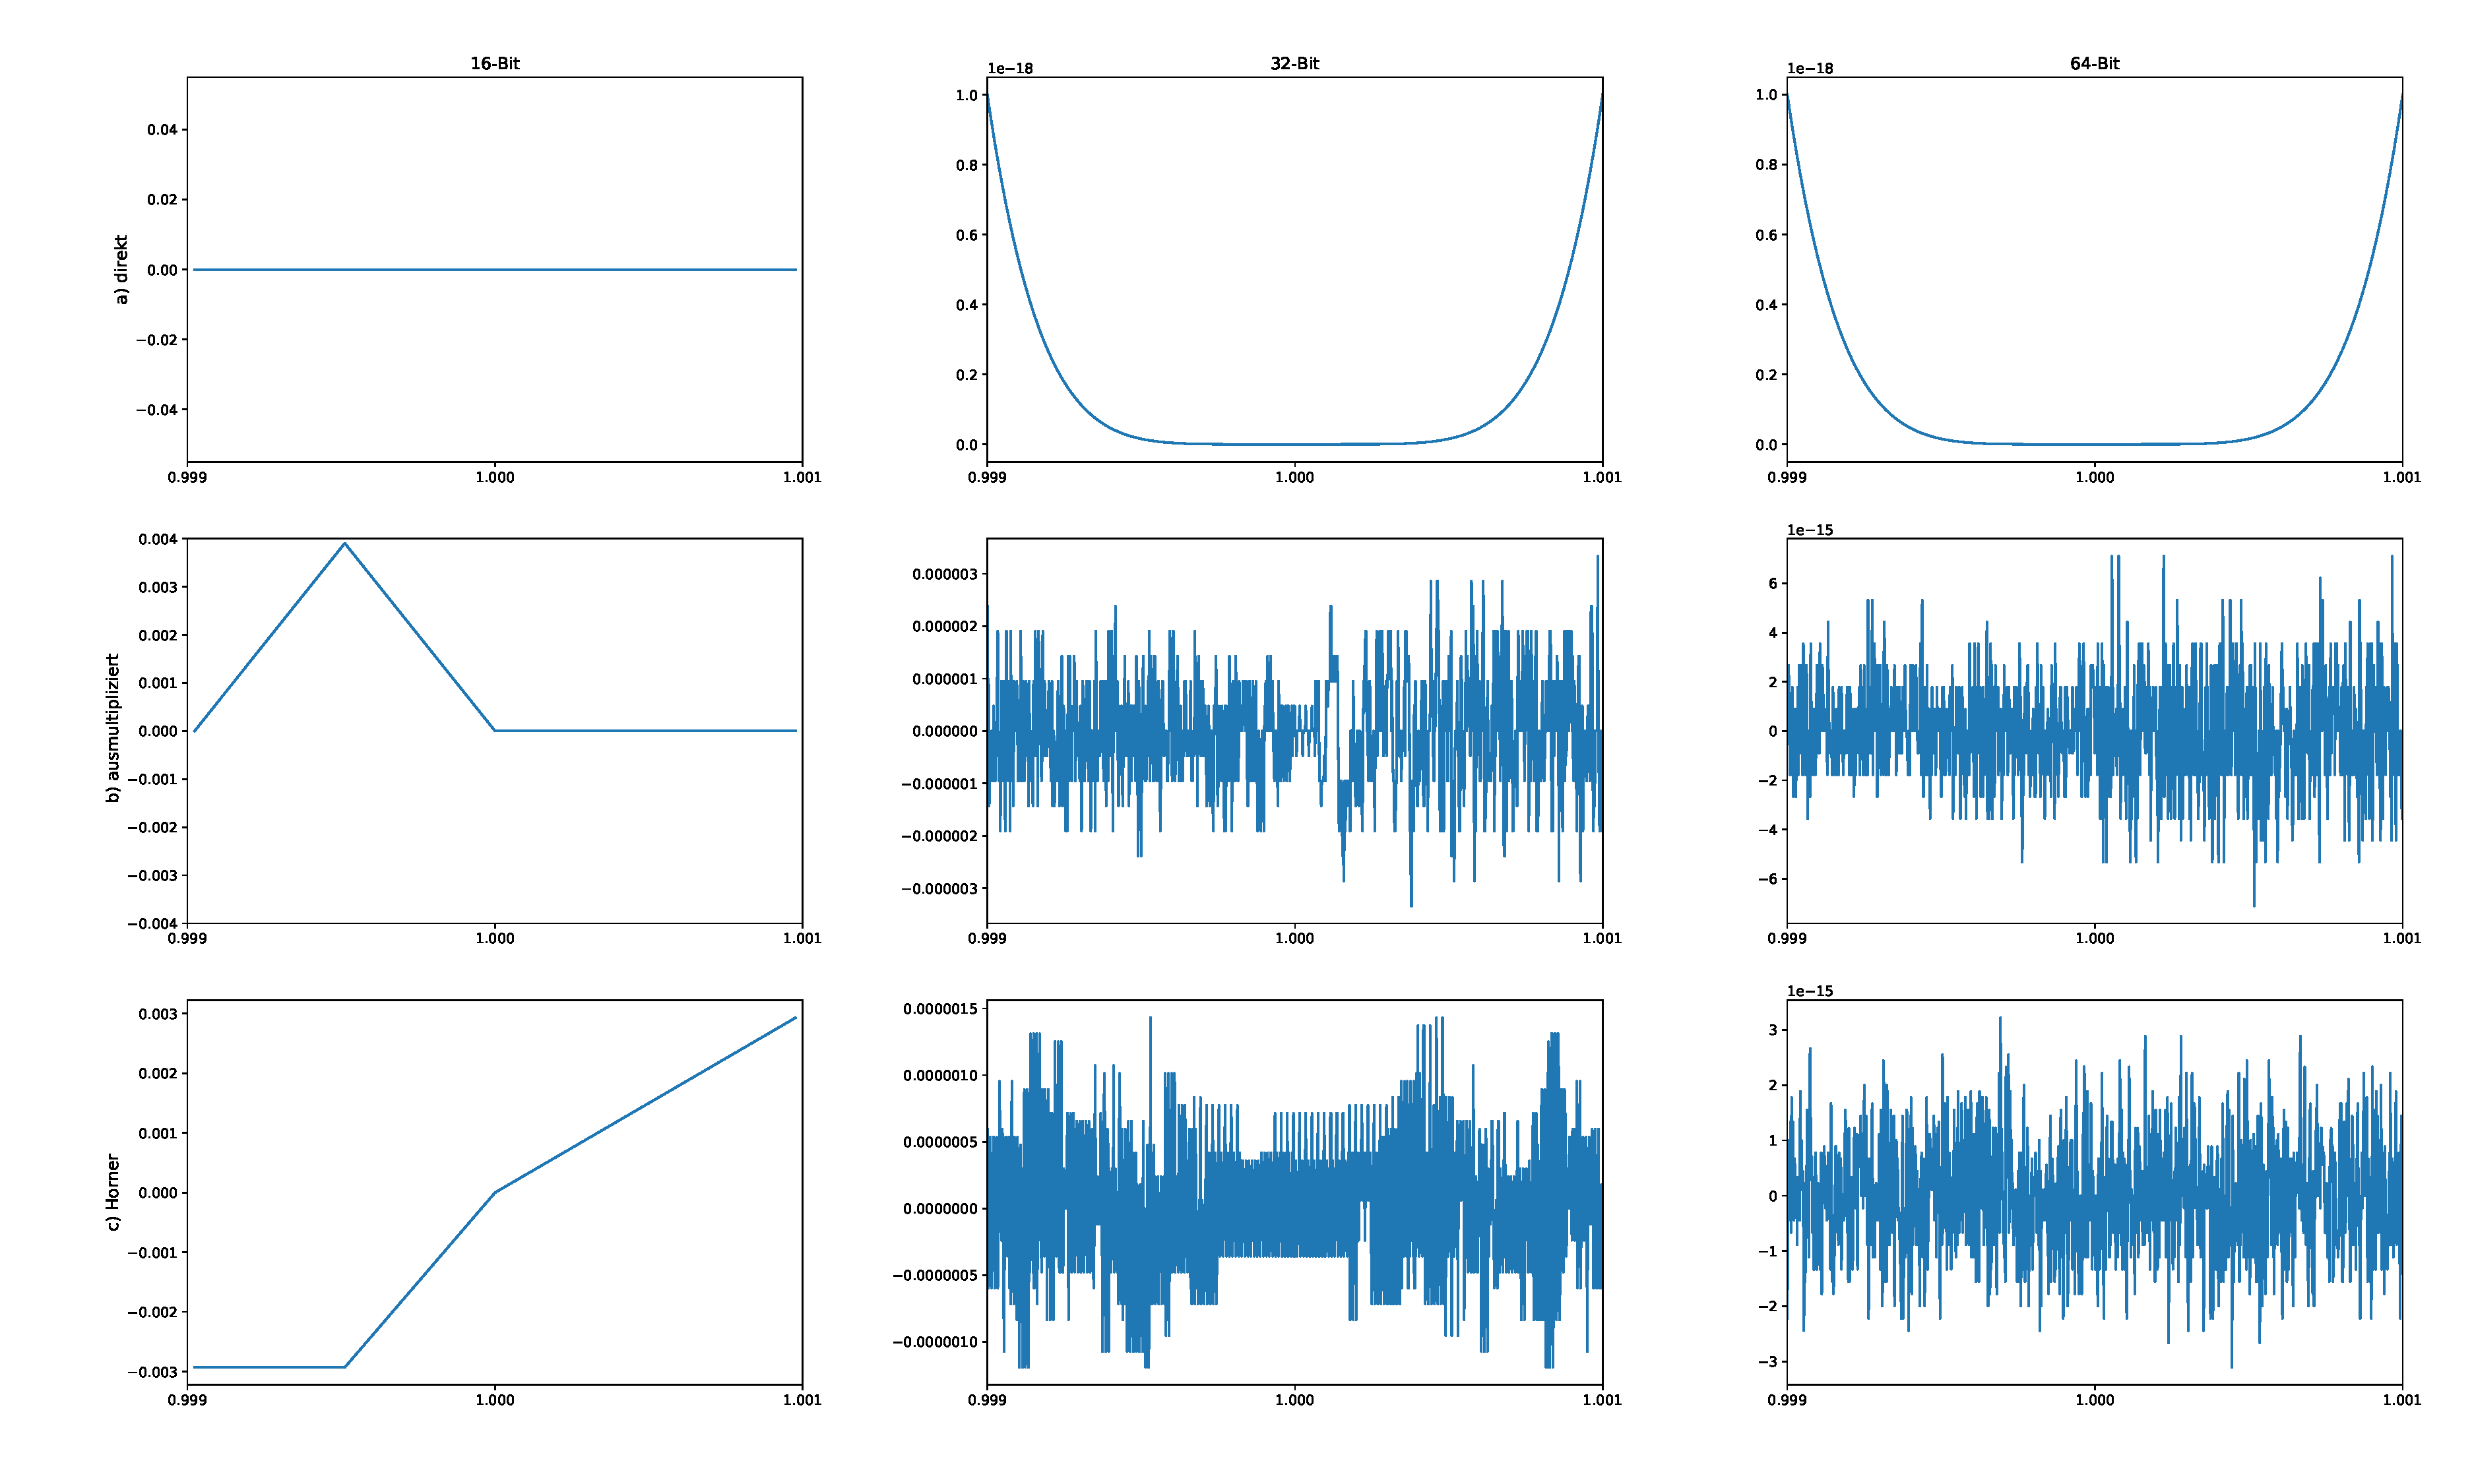
\includegraphics[width=\textwidth]{../A01/A1.pdf}
    \caption{Ergebnisse zu Aufgabe 1.}
    \label{fig:a1}
\end{figure}
Unsere Ergebnisse zu Aufgabe 1 finden sich in Abbildung~\ref{fig:a1}. Wir gehen davon aus, dass ihr unsere Abgaben zum Korrigieren nicht ausdruckt, darum sollte die Darstellung so mit zoomen gut funktionieren und übersichtlicher sein, als alles einzeln darzustellen. In der ersten Zeile ist das Ergebnis von $(1-x)^6$ in unveränderter Form dargestellt, in der zweiten Zeile die ausmultiplizierte Form und in der dritten Zeile wird mittels Hornerschema ausgewertet. Die Spalten von links nach rechts verwenden 16-Bit, 32-Bit und 64-Bit Gleitkommazahlen. 

Allgemein ist zu sagen, dass wie erwartet mit erhöhter Genauigkeit der Gleitkommazahlen auch die Genauigkeit des Ergebnisses zunimmt. Eine Ausnahme ist mit der faktorisierten Form aus a) gegeben, denn hier liefern bereits 32-Bit Gleitkommazahlen das exakte Ergebnis. Die faktorisierte Form ist mit Abstand die beste, da sich die Fehler hier nicht akkumulieren und insgesamt weniger Rechenoperationen durchgeführt werden müssen. Bei den beiden anderen Formen müssen deutlich mehr Rechenoperationen durchgeführt werden wobei sich die Fehler fortpflanzen.

\FloatBarrier
\section*{Aufgabe 2}
\subsection*{a)}
Der analytische Grenzwert ergibt mit Hilfe des Satz von \textsc{L'Hospital} sich wie folgt:
\begin{equation}
    \lim_{x \to 0} \frac{\sqrt{9 - x}- 3}{x} = \lim_{x \to 0}\frac{-\frac{1}{2}(9 - x)^{-\frac{1}{2}}}{1} = -\frac{1}{6}\,.
    \label{eqn:2a}
\end{equation}

\subsection*{b)}
\begin{figure}
    \centering
    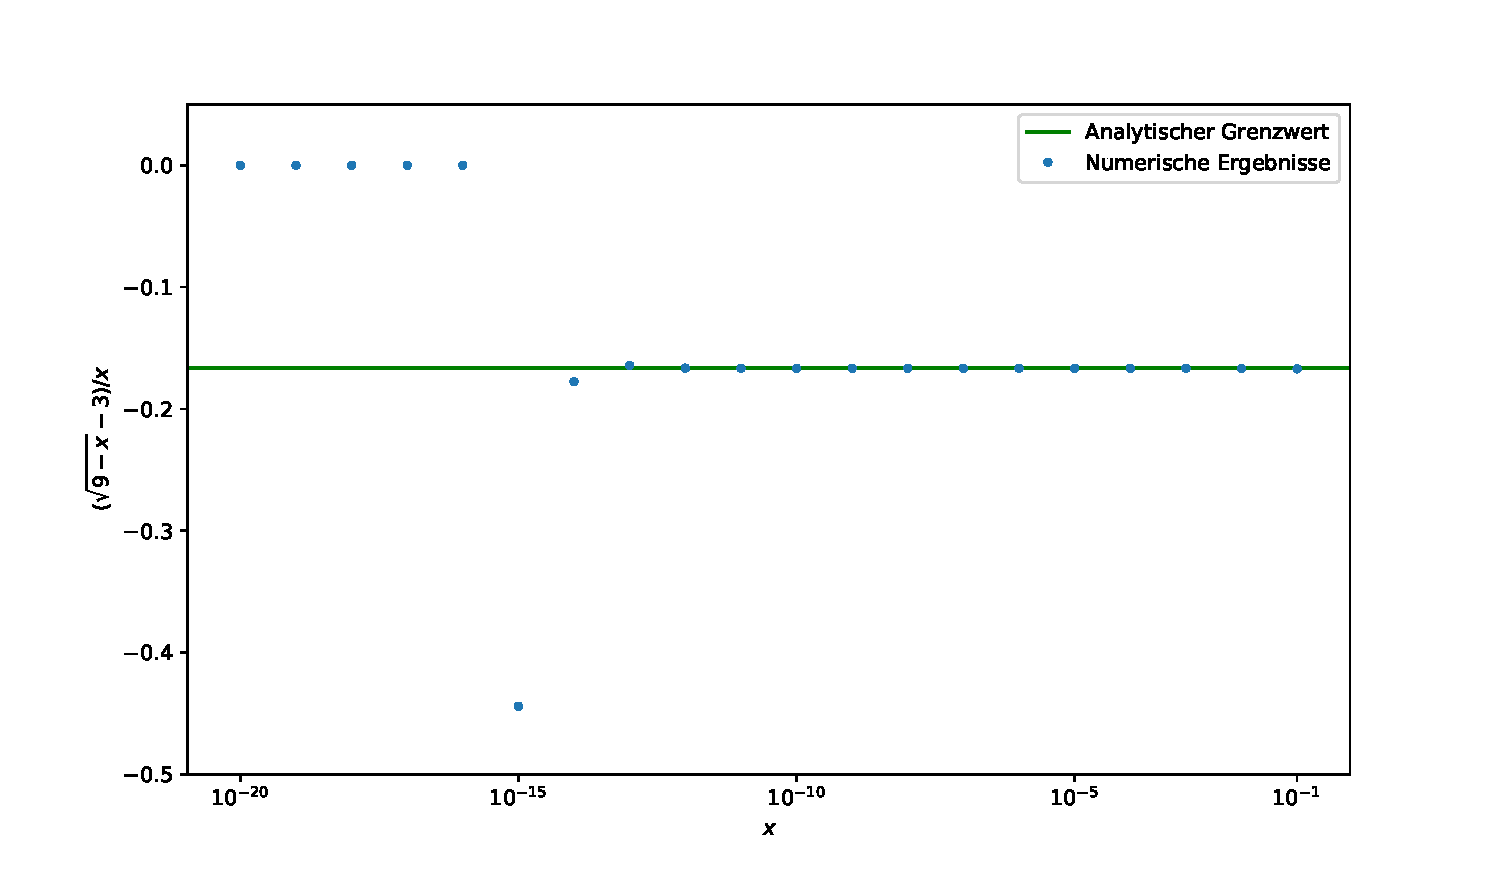
\includegraphics[width=\textwidth]{../A02/A2.pdf}
    \caption{Vergleich des analytisches Grenzwertes mit dem numerischen Ergebnis.}
    \label{fig:2b}
\end{figure}
Der verwendete \textsc{Python} Datentyp \textit{float} verwendet standardmäßig 53 Bit Präzession damit wird eine Rechnergenauigkeit von $10^{-15}$ erreicht. Wie in Abbildung~\ref{fig:2b} gut zu erkennen ist, führt dies dazu, dass bei der Differenzbildung im Fall von $x < 10^{-15}$ das Ergebnis gezwungener Maßen auf exakt 9 gerundet wird, und der Zähler somit 0 ergibt. Anschließend wird durch $0 < x < 10^{-15}$ geteilt was zum Gesamtergebnis 0 führt. Für $x > 10^{-15}$ tritt dieses Rundungsproblem noch nicht auf, und das Ergebnis liegt sehr nahe am analytischen Grenzwert, da der Grenzwert schnell konvergiert.

\FloatBarrier
\section*{Aufgabe 3}
\begin{figure}
    \centering
    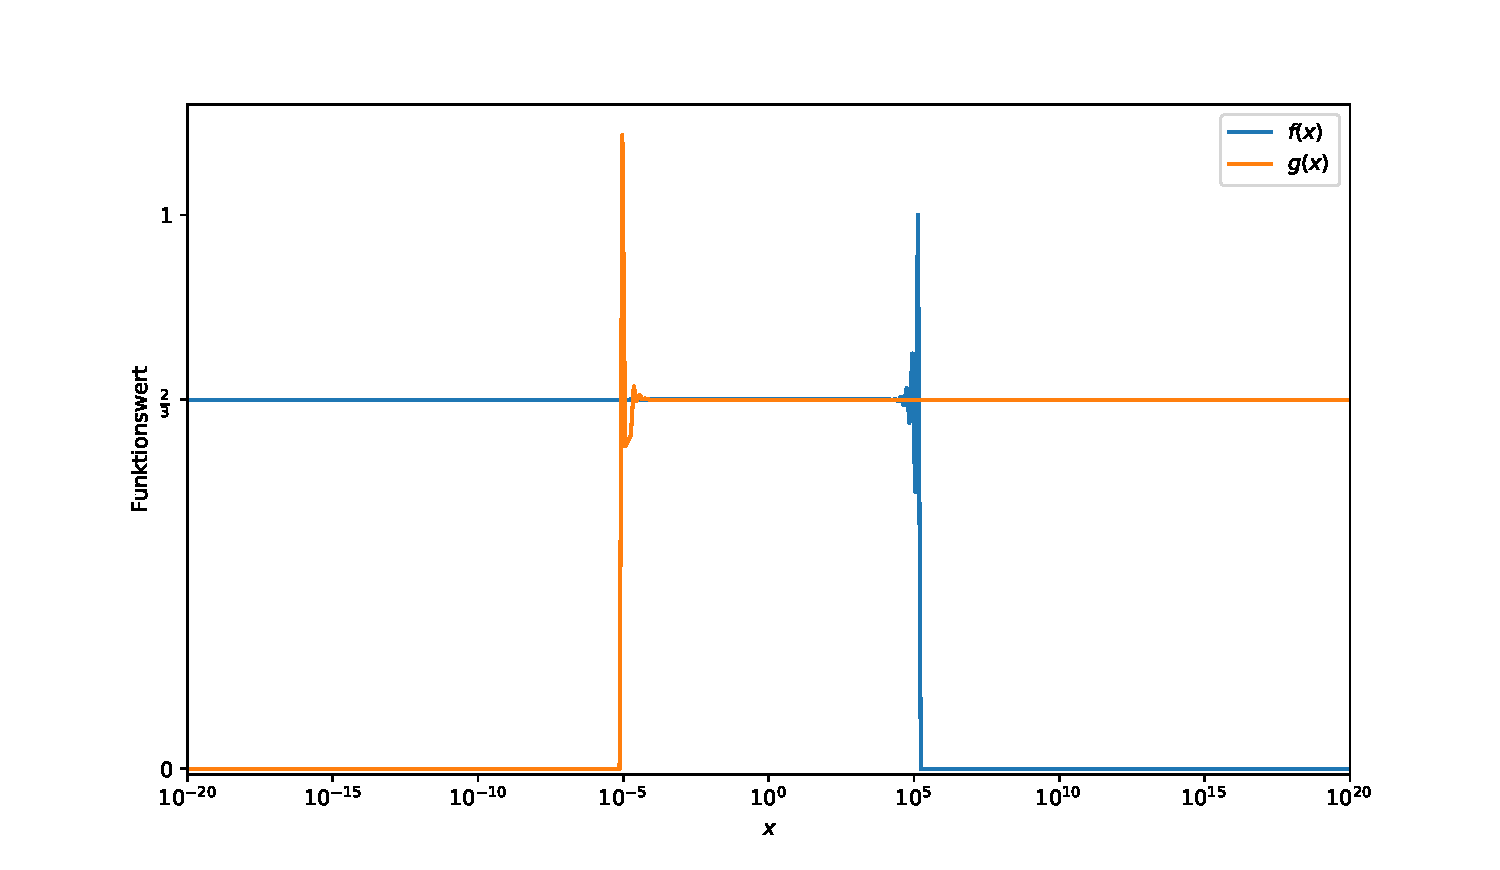
\includegraphics[width=\textwidth]{../A03/A3.pdf}
    \caption{Vergleich der numerischen Ergebnisse.}
    \label{fig:a3}
\end{figure}

Es gilt
\begin{equation}
    f(x) = g(x) = \frac{2}{3},\quad \forall x\,.
\end{equation}
Bis zur Stelle $x \approx 10^{4}$ nimmt $f$ den analytisch korrekten Wert an und ist für $x > 10^{5}$ null. In der Darstellung $g$ ist das Verhalten umgekehrt: Hier ist das numerische Ergebnis für etwa $x < 10^{-5}$ gleich Null und ab ungefähr $x = 10^{-4}$ gleich dem analytischen Wert. Das Verhalten für $f$ lässt sich dadurch erklären, dass für große $x$ am Rande der Rechnergenauigkeit die Terme $\pm \frac{1}{3}$ verloren gehen, sodass sich $x^3 - x^3 = 0$ ergibt. Im Fall von $g$ tritt das umgekehrte Problem auf, denn hier wird für sehr kleine $x$ $\frac{x^3}{3}$ zu klein gegenüber 3 um bei der gegebenen Rechnergenauigkeit dargestellt werden zu können. Es ergibt sich so $3 - 3 = 0$.

\FloatBarrier
\section*{Aufgabe 4}
\begin{equation}
    \frac{\mathrm{d}\sigma}{\mathrm{d}\Omega} = \frac{\alpha^2}{s}
    \left(\frac{2+\sin^2\left(\theta\right)}{1-\beta^2 \cos^2\left(\theta\right)}\right) =: f\left(\theta\right)\\
    \label{eqn:dsdo}
\end{equation}
\subsection*{a)}
Die Funktion ist numerisch instabil, da $\beta \approx 1$ gilt und damit
\begin{equation}
    1 - \beta^2 \cos^2\left(n\cdot\mathrm{\pi}\right) \approx 0 \qquad\forall n \in \mathbb{Z}
\end{equation}
gilt.
An den Stellen, an denen $\theta$ ein ganzzahliges Vielfaches von $\mathrm{\pi}$ ist, wird dann durch fast Null geteilt, was schnell zu Rundungsfehlern führt.
\subsection*{b)}
Die folgende Umformung sorgt dafür, dass nicht mehr durch fast Null geteilt wird:
\begin{align}
    \frac{\mathrm{d}\sigma}{\mathrm{d}\Omega} &= \frac{\alpha^2}{s}
    \left(\frac{2+\sin^2\left(\theta\right)}{1-\beta^2 \cos^2\left(\theta\right)}\right) =: f\left(\theta\right)\\
    \Leftrightarrow &= \frac{\alpha^2}{s} \left(\frac{2+\sin^2\left(\theta\right)}{\sin^2\left(\theta\right)+\cos^2\left(\theta\right)-\beta^2 \cos^2\left(\theta\right)}\right)\\
    \Leftrightarrow &= \frac{\alpha^2}{s} \left(\frac{2+\sin^2\left(\theta\right)}{\sin^2\left(\theta\right)+\left(1-\beta^2\right)\cos^2\left(\theta\right)}\right)\\
    \Leftrightarrow &= \frac{\alpha^2}{s} \left(\frac{2+\sin^2\left(\theta\right)}{\sin^2\left(\theta\right)+\frac{1}{\gamma^2}\cos^2\left(\theta\right)}\right)\\
    \Leftrightarrow &= \frac{\alpha^2}{s} \gamma^2 \left(\frac{2+\sin^2\left(\theta\right)}{\gamma^2\sin^2\left(\theta\right)+\cos^2\left(\theta\right)}\right)
    \label{eqn:dsdogut}
\end{align}
\subsection*{c)}
\begin{figure}
    \centering
    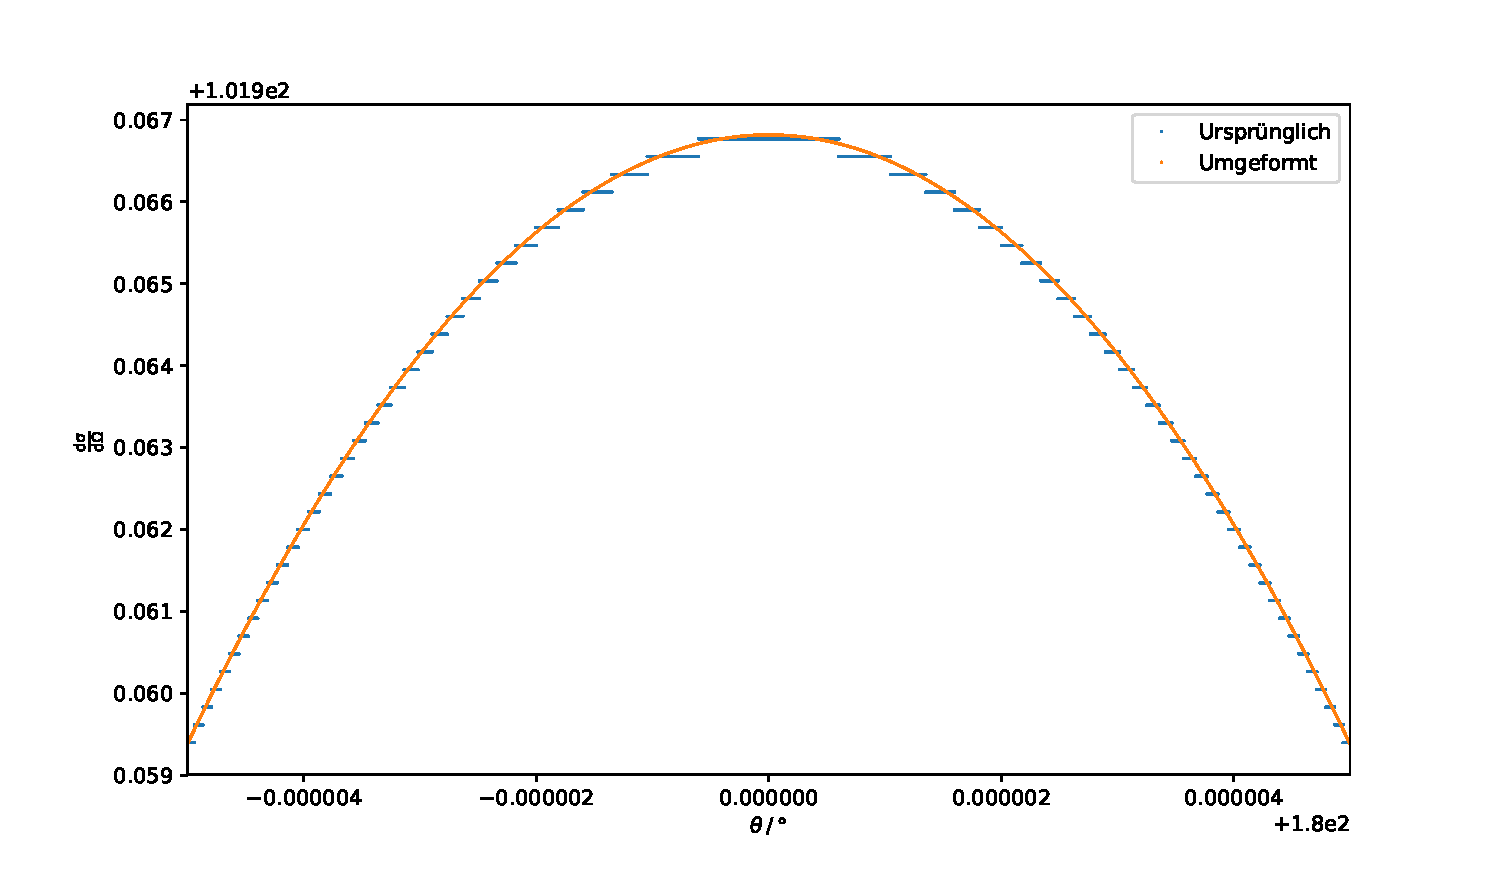
\includegraphics[width=\textwidth]{../A04/A4_stab.pdf}
    \caption{Vergleich der numerisch stabilen und instabilen Form.}
    \label{fig:4c}
\end{figure}
Die Unterschiede zwischen den beiden Formen \eqref{eqn:dsdo} und \eqref{eqn:dsdogut} sind in Abbildung~\ref{fig:4c} gut zu erkennen.
Dabei wurden die ursprüngliche Funktion in blau und die umgeformte Funktion in orange gezeichnet in dem Bereich um $\theta \approx 0\cdot\mathrm{\pi}$ geplottet.
Es ist gut zu erkennen, dass die ursprüngliche Form Plateaus bildet.
Sie liefert also für mehrere Werte von $\theta$ den gleichen Wert und springt dann am Ende des Plateaus plötzlich auf einen anderen Wert.
Dieses Verhalten ist bei der umgeformten Funktion nicht mehr zu beobachten.
\subsection*{d)}
\begin{equation}
    \begin{split}
        f'\left(\theta\right) &= \frac{-2 \sin\left(\theta\right)\cos\left(\theta\right) \left(1+\beta^2\right)}{\left(1-\beta^2 \cos^2\left(\theta\right)\right)^2} \\
        \\
        \Rightarrow K &= \left| \theta  \frac{f'\left(\theta\right)}{f\left(\theta\right)}\right| \\
        &= \left| \theta  \frac{-2 \sin\left(\theta\right)\cos\left(\theta\right)\left(1+\beta^2\right)\left(1-\beta^2 \cos^2\left(\theta\right)\right)}
        {\left(1-\beta^2 \cos^2\left(\theta\right)\right)^2 \left(2+\sin^2\left(\theta\right)\right)} \right| \\
        &= \left| \theta  \frac{-2 \sin\left(\theta\right)\cos\left(\theta\right)\left(1+\beta^2\right)}{\left(1-\beta^2 \cos^2\left(\theta\right)\right) \left(2+\sin^2\left(\theta\right)\right)}\right|
    \end{split}
    \label{eqn:K}
\end{equation}
\subsection*{e)}
\begin{figure}
    \centering
    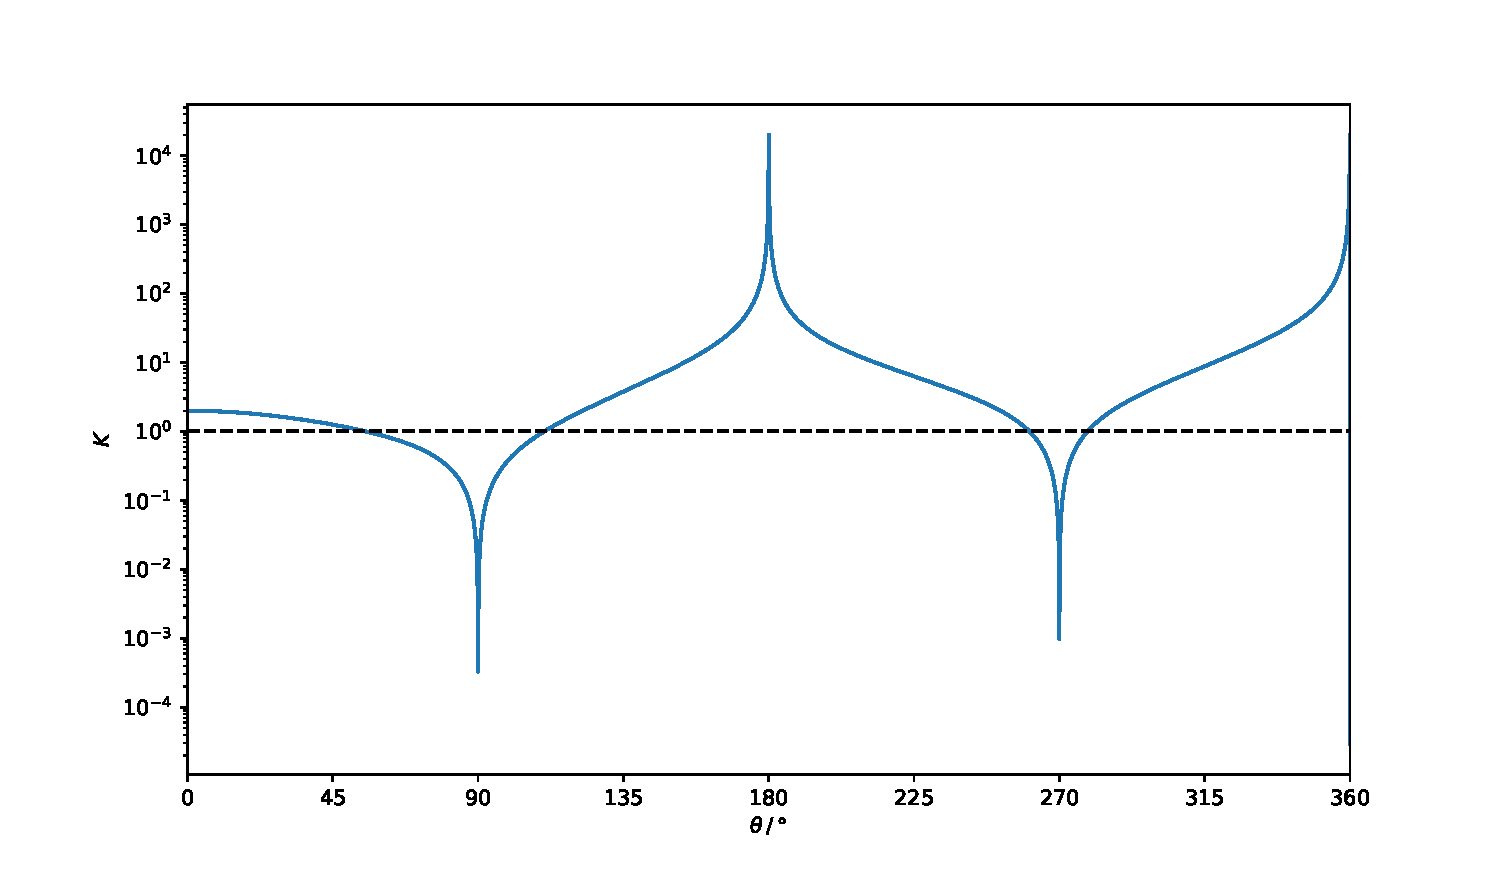
\includegraphics[width=\textwidth]{../A04/A4_kond.pdf}
    \caption{Grafische Darstellung des Verlaufs der Konditionszahl.}
    \label{fig:K}
\end{figure}
Ein Problem hat für $K<1$ eine Fehlerdämpfung und für $K>1$ eine Fehlerverstärkung.
Die Bereiche sind in Abbildung~\ref{fig:K} durch die gestrichelte Linie abgetrennt.
Auffällig ist, dass das Problem bei $\theta = \frac{\mathrm{\pi}}{2}$ besonders gut, und bei $\theta = \mathrm{\pi}$ besonders schlecht konditioniert ist.
\end{document}
